% ============================================================
\chapter{Introduction to Time Series}
\label{ch:intro}
% ============================================================

\section{Motivating example}
The daily closing price of the CAC~40 index from 2000 to 2024 exhibits a trend, cycles, and time-varying volatility. Unlike iid data, each observation depends on the preceding ones. Time series analysis exploits this dependence.

\section{Fundamental definitions}

\begin{definition}[Time series]\index{time series}
A \textbf{time series} (or \textbf{discrete-time stochastic process}) is a sequence of random variables $(X_t)_{t\in\Z}$ defined on a probability space $(\Omega,\mathcal{F},P)$. A \textbf{realisation} (or sample path) is an observed sequence $(x_1,\ldots,x_n)$.
\end{definition}

\begin{definition}[White noise]\index{white noise}
A \textbf{white noise} $(\eps_t)$ is a sequence of random variables such that:
\begin{enumerate}
\item $\E[\eps_t]=0$ for all $t$,
\item $\Var(\eps_t)=\sigma^2$ for all $t$,
\item $\Cov(\eps_t,\eps_s)=0$ for $t\neq s$.
\end{enumerate}
Notation: $\eps_t\sim\mathrm{WN}(0,\sigma^2)$. If, in addition, the $\eps_t$ are Gaussian, it is called a \textbf{Gaussian white noise}.
\end{definition}

\begin{definition}[Strong white noise]\index{white noise!strong}
A \textbf{strong white noise} is an iid sequence of random variables with zero mean and finite variance. A (weak) white noise only requires uncorrelatedness, not independence.
\end{definition}

\section{Components of a time series}

\begin{definition}[Classical decomposition]\index{decomposition}
A time series is often decomposed as:
\[
X_t = T_t + S_t + R_t,
\]
where $T_t$ is the \textbf{trend}, $S_t$ the \textbf{seasonality} (periodic component), and $R_t$ the \textbf{residual} (random component).

\textbf{Multiplicative} model: $X_t = T_t\cdot S_t\cdot R_t$ (common when the seasonal amplitude grows with the level).
\end{definition}

\section{Lag and difference operators}

\begin{definition}[Lag operator]\index{lag operator}
The \textbf{lag operator} $B$ (or \emph{backshift operator}) is defined by:
\[
BX_t = X_{t-1}, \quad B^k X_t = X_{t-k}.
\]
The \textbf{difference operator} is $\nabla = 1-B$: $\nabla X_t = X_t - X_{t-1}$.
\end{definition}

\begin{remark}
Polynomials in $B$ are manipulated as ordinary polynomials. For example, $(1-\phi B)X_t = \eps_t$ can be written as $X_t - \phi X_{t-1} = \eps_t$.
\end{remark}

\section{Examples of time series}

\begin{example}[Random walk]\index{random walk}
$X_t = X_{t-1} + \eps_t$ with $\eps_t\sim\mathrm{WN}(0,\sigma^2)$. Then $X_t = X_0 + \sum_{i=1}^t \eps_i$ and $\Var(X_t) = t\sigma^2 \to \infty$: the random walk is \textbf{not stationary}.
\end{example}

\begin{example}[Linear trend + noise]
$X_t = a + bt + \eps_t$. Not stationary (the mean $\E[X_t] = a+bt$ depends on $t$).
\end{example}

\begin{example}[Seasonal series]
Monthly temperatures: period $s=12$. The component $S_t$ is modelled by trigonometric functions or monthly indicator variables.
\end{example}

\section{Visualisation}

\begin{center}
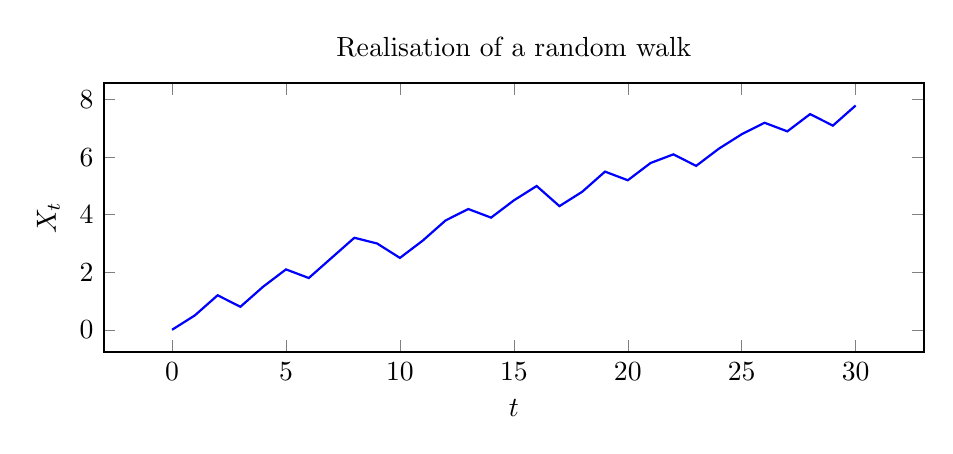
\begin{tikzpicture}
\begin{axis}[
  width=12cm, height=5cm, xlabel={$t$}, ylabel={$X_t$},
  title={Realisation of a random walk},
  no markers, thick
]
\addplot[blue] coordinates {
(0,0)(1,0.5)(2,1.2)(3,0.8)(4,1.5)(5,2.1)(6,1.8)(7,2.5)(8,3.2)
(9,3.0)(10,2.5)(11,3.1)(12,3.8)(13,4.2)(14,3.9)(15,4.5)(16,5.0)
(17,4.3)(18,4.8)(19,5.5)(20,5.2)(21,5.8)(22,6.1)(23,5.7)(24,6.3)
(25,6.8)(26,7.2)(27,6.9)(28,7.5)(29,7.1)(30,7.8)
};
\end{axis}
\end{tikzpicture}
\end{center}

\begin{center}
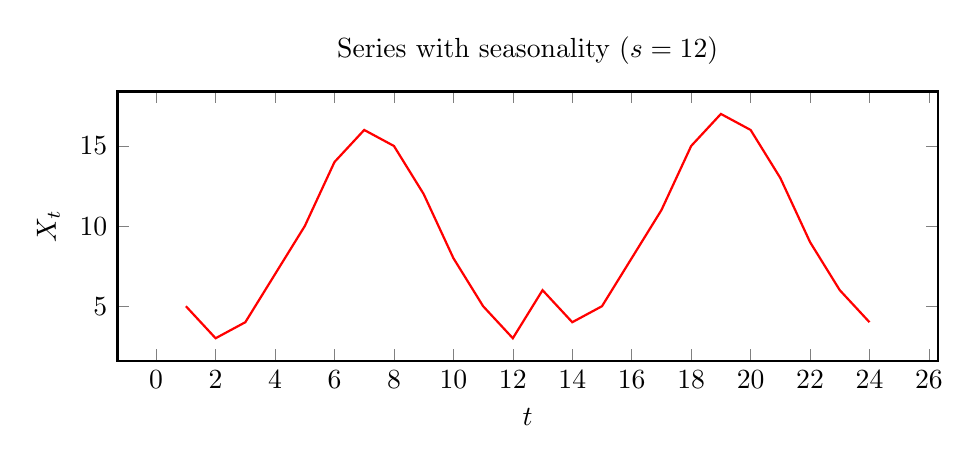
\begin{tikzpicture}
\begin{axis}[
  width=12cm, height=5cm, xlabel={$t$}, ylabel={$X_t$},
  title={Series with seasonality ($s=12$)},
  no markers, thick
]
\addplot[red] coordinates {
(1,5)(2,3)(3,4)(4,7)(5,10)(6,14)(7,16)(8,15)(9,12)(10,8)(11,5)(12,3)
(13,6)(14,4)(15,5)(16,8)(17,11)(18,15)(19,17)(20,16)(21,13)(22,9)(23,6)(24,4)
};
\end{axis}
\end{tikzpicture}
\end{center}

\section{Implementation}

\begin{codeblock}[title=\textbf{Python}]
\begin{minted}{python}
import numpy as np
import pandas as pd
import matplotlib.pyplot as plt

# Simuler une marche aléatoire
np.random.seed(42)
n = 500
eps = np.random.normal(0, 1, n)
rw = np.cumsum(eps)

# Simuler un AR(1)
phi = 0.8
ar1 = np.zeros(n)
for t in range(1, n):
    ar1[t] = phi * ar1[t-1] + eps[t]

# Charger des données réelles (exemple : AirPassengers)
# url = 'https://raw.githubusercontent.com/jbrownlee/Datasets/master/airline-passengers.csv'
# df = pd.read_csv(url, parse_dates=['Month'], index_col='Month')

fig, axes = plt.subplots(2, 1, figsize=(12, 6))
axes[0].plot(rw, lw=0.8)
axes[0].set_title('Marche aléatoire')
axes[0].set_xlabel('t')

axes[1].plot(ar1, lw=0.8, color='red')
axes[1].set_title('AR(1) avec $\\phi=0.8$')
axes[1].set_xlabel('t')

plt.tight_layout()
plt.savefig('ch01_intro.pdf')
plt.show()
\end{minted}
\end{codeblock}

\section{Exercises}

\begin{exercise}[$\star$]
Simulate 1000 realisations of a random walk of length $n=200$. Plot 10 sample paths on the same graph. Compute the empirical variance of $X_{200}$.
\end{exercise}

\begin{exercise}[$\star$]
Load the \texttt{AirPassengers} series. Visually identify the trend, seasonality, and increasing volatility. Suggest an additive or multiplicative model.
\end{exercise}

\begin{exercise}[$\star\star$]
Show that if $X_t = X_{t-1}+\eps_t$ (random walk), then $\Var(X_t)=t\sigma^2$ and $\Corr(X_t,X_s)=\sqrt{\min(t,s)/\max(t,s)}$ for $t,s>0$.
\end{exercise}

\begin{exercise}[$\star\star\star$ -- Project]
Download the daily prices of a stock (e.g.\ Apple) over 5 years. Decompose the series into trend, seasonality, and residual. Compute the log-returns $r_t=\ln(P_t/P_{t-1})$ and analyse their statistical properties.
\end{exercise}

\begin{keyformulas}
\begin{align*}
BX_t &= X_{t-1}, \quad \nabla X_t = X_t - X_{t-1} \\
X_t &= T_t + S_t + R_t \quad \text{(additive decomposition)} \\
\text{Random walk} &: X_t = X_{t-1}+\eps_t, \quad \Var(X_t)=t\sigma^2
\end{align*}
\end{keyformulas}
